\clearpage
\thispagestyle{empty}

\movetoevenpage
\small\MyriadPro\itshape
\label{colaboradores}

\noindent{}SOBRE O AUTOR\\

\begin{center}
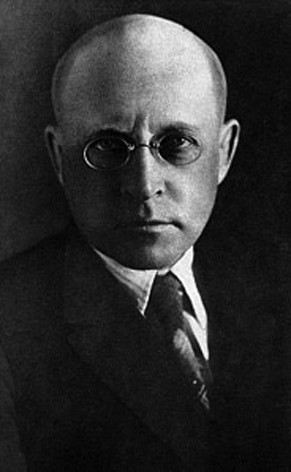
\includegraphics[width=4cm]{./autor.jpg}
\end{center}

\epigraph{{\slsc{No fim de 1987, um pouco depois de voltar de Estocolmo, onde fora
receber o Nobel de literatura, Joseph Brodsky falava a um grupo de
estudantes e professores da Universidade de Harvard. O escritor Arkádi
Lvóv lembra o episódio no jornal:\\
— Qual dos escritores\ldots{}\\
Brodsky nem terminou de ouvir a pergunta:\\
— Minha altivez é a poesia.\\
— Mesmo assim, quem o senhor considera o maior escritor russo
pós-revolucionário?\\
Brodsky refletiu. Ouviam-se vozes de todos os lados:\\
— Bulgákov, Platónov, Bábel, Zóschenko\ldots{}\\
— Dobýtchin — proferiu Brodsky rapidamente. — Leonid
Dobýtchin.}}}{(Extraído de um artigo de V. Mechkóv, publicado em {\slsc{Gazeta da
Cidade}}, Eupatória, Ucrânia, ago–out, 2007, nº 29–39)}

O nome de Leonid Dobýtchin (1894–1936), hoje aclamado por literatos
russos, foi redescoberto depois de 1990. Dobýtchin enfrentou uma vida
repleta de dificuldades. Trabalhou como estatístico em regiões do norte
da Rússia, dividindo quartos de solteiro com a mãe, uma parteira, e três
irmãos. Viveu os últimos de sua vida em Leningrado (atual São
Petersburgo).

A morte do escritor, em 1936, provável suicídio, ocorreu no momento em
que Stálin declarou guerra contra o formalismo. Ser tachado de
formalista e politicamente míope, como Dobýtchin o foi após a publicação
da novela {\slsc{A Cidade Ene}} (1935), era na época uma acusação
gravíssima. Ele defendeu-se dela numa reunião na União dos Escritores de
Leningrado e desapareceu no dia seguinte.

Em vida, além da novela, publicou duas coletâneas de contos,
{\slsc{Encontros com Liz}} (1927) e {\slsc{O retrato}} (1931) --- reunidas em
{\slsc{Encontros com Liz e outras histórias}} (ed. Kalinka, 2009). Escreveu ainda
{\slsc{Os Selvagens}} (1989) e {\slsc{O Clã do Churka}} (1993), este que
recebeu o prêmio “Internacional Book of the Year” do {\slsc{Times
Literary Supplement}} de 1994.

\bigskip

\noindent{}SOBRE A COLEÇÃO\\

A coleção “Contos russos modernos (1900-1930)” traz escritos das
primeiras três décadas do século \scalebox{.8}{XX} e privilegia uma série de autores
russos sobrepujada pela censura stalinista. Esse grupo de escritores e
poetas em geral deixou de ser publicado nos anos 1930 e foi redescoberto
após o fim da \scalebox{.8}{URSS}. Como uma cápsula do tempo, escondida no subsolo, são
testemunhas literárias de um passado ainda velado, porém muito vivo,
escrevendo numa linguagem não raro inovadora que com certeza haverá de
interessar aos leitores.

\pagebreak

\noindent{}COLABORADORES\\

\noindent{}MOISSEI MOUNTIAN, nascido na Moldávia (\scalebox{.8}{URSS}), é formado em engenharia civil. Em 1972, mudou"-se com sua esposa, Sofia Mountian, para o Brasil,
onde em 2008 fundou com sua filha Daniela a editora Kalinka e começou a
trabalhar como tradutor. É parte do conselho editorial da Kalinka, tendo
trazido nomes como Fiódor Sologub, Leonid Dobýtchin e Friedrich
Gorenstein aos leitores brasileiros. Foi indicado duas vezes ao Prêmio
Jabuti pelas traduções de {\slsc{O diabo mesquinho}}, de Fiódor Sologub
(Kalinka, 2008) e {\slsc{“Os sonhos teus vão acabar contigo”: prosa,
poesia, teatro}}, de Daniil Kharms (Kalinka, 2103, com Aurora Fornoni
Bernardini e Daniela Mountian). Também traduziu {\slsc{Encontros com Liz
e outras histórias}}, de Leonid Dobýtchin (Kalinka, 2009), {\slsc{Diário
de um escritor (1873): Meia carta de um sujeito}}, de Fiódor Dostoiévski
(Hedra, 2016), e {\slsc{A ressurreição do lariço: Contos de Kolimá 5}}, de
Varlam Chalámov (Ed. 34, 2016), os dois últimos em parceria com Daniela.
Com Irineu Franco Perpetuo verteu {\slsc{Salmo}}, de Friedrich Gorenstein
(indicado ao prêmio de tradução “Lendo a Rússia”, do Instituto de
Tradução de Moscou).

\medskip

\noindent{}DANIELA MOUNTIAN é tradutora, designer e criadora da Kalinka, de­dicada
à cultura russa. Fez pela \scalebox{0.8}{USP} graduação em história, mestrado sobre
Fiódor Sologub e doutorado"-sanduíche sobre Daniil Kharms, com estágio de
um ano na Casa de Púchkin, em São Petersburgo. Atualmente é
pós"-doutoranda do Departamento de Teoria Literária e Literatura
Comparada (\scalebox{0.8}{USP}), com apoio da \scalebox{0.8}{FAPESP} (processo 2017/24139-9), com a pesquisa “Literatura infantil
russa e brasileira: uma análise comparada (1919-1943)”. Além dos livros
vertidos em parceria com Moissei Mountian, traduziu com Yulia Mikaelian
{\slsc{O ofício}} e {\slsc{O compromisso}}, ambos de Serguei Dovlátov
(Kalinka, 2017, 2019).


\medskip

\noindent{}VALÉRI NIKOLÁIEVITCH SÁJIN, nascido em 1946 em Leningrado, é crítico
literário, autor de livros e artigos sobre literatura e cultura russa
dos séculos \scalebox{.8}{XVIII} ao \scalebox{.8}{XX}.
Membro da União dos Escritores de São
Petersburgo desde 1994. Enquanto estudava na escola da juventude
operária, trabalhou, entre 1961 e 1964, como serralheiro ferramenteiro
numa fábrica de equipamentos radiotécnicos. A partir de 1964 cursou a
Faculdade de Língua e Literatura Russa do Instituto Pedagógico Estatal
de Leningrado A. I. Herzen, finalizada em 1968. Entre 1968 e 1992 (com
intervalo para o serviço militar de 1969 a 1970) foi colaborador
científico do Departamento de Manuscritos da Biblioteca Pública Estatal
M. E. Saltykóv"-Schedrin (atual Biblioteca Nacional da Rússia). De 1998 a
2001 foi coeditor da revista {\slsc{Trimestre da cultura e filologia
russa}}. É autor dos livros: {\slsc{Livros de verdade amarga}} (Moscou, ed.
{\slsc{Kniga}}, 1989); {\slsc{Força do destino. Uma crônica documental do
ano 1861}} (São Petersburgo, {\slsc{Aleteia}}, 2010). Organizou as
primeiras {\slsc{Obras completas de Daniil Kharms}} em seis tomos (São
Petersburgo, {\slsc{Akademítcheskoi Proiekt}}, 1997-2001) e várias
coletâneas de suas obras; uma coletânea de poemas de B. Ch. Okudjava
(série Biblioteca do Poeta, São Petersburgo, {\slsc{Akademítcheskoi
Proiekt}}, 2001); as {\slsc{Obras completas de I. S. Barkóv}} (série
Biblioteca do Poeta, São Petersburgo, {\slsc{Akademítcheskoi Proiekt}},
2004); a coletânea das obras de L. S. Lipávski {\slsc{Estudo do terror}}
(Moscou, {\slsc{Ad Marginem}}, 2005); {\slsc{Diário de L. V. Chapórina}} em
2 tomos (Moscou, {\slsc{Nóvoie Literatúrnoie Obozriénie}}, 2012); e em
parceria com A. L. Dmitrenko o livro {\slsc{Daniil Kharms pelo olhar de
seus contemporâneos: Reminiscências. Diários. Cartas}} (São Petersburgo,
Vita Nova, 2019).

\medskip

\noindent{}KARINA AOKI é formada em arquitetura pela \scalebox{.8}{FAU-USP}. Atuou como diretora de arte e coordenadora de estúdio da São Paulo Criação – Rafic Farah
durante 8 anos, atendendo clientes como Mitsubishi Motors do Brasil,
Fundação Roberto Marinho, Fast Shop, Casa do Saber, Escola da Cidade,
Museu de Arte Brasileira da \scalebox{.8}{FAAP}, restaurantes Arabia, Spot e Ritz,
marcas de moda Maria Bonita, Mandi, Lucy in the Sky e Brooksfield Donna,
cinema \scalebox{.8}{HSBC}/Belas Artes, e o designer Carlos Motta. Foi também editora
de arte da revista {\slsc{Casa Vogue}} (Edições Globo Condé Nast) por 6 anos e
supervisora de arte do departamento de literatura da editora \scalebox{.8}{FTD}
Educação, sendo responsável por cerca de 70 títulos. Atualmente
desenvolve projetos independentes nas áreas de identidade visual,
embalagem, expografia e editorial.

\medskip

\noindent{}PAULO HENRIQUE POMPERMAIER é graduado em Jornalismo pela Faculdade Cásper Líbero e graduando em Letras pela \scalebox{0.8}{USP}. Como repórter atuou na Revista {\slsc{Cult}} e atualmente é editor"-assistente da Hedra.

\afterpage{\blankpage}

\newpage
\pagestyle{empty}
\MyriadPro

\footnotesize{
\noindent{}CATÁLOGO DA EDITORA KALINKA\\[5pt]

\noindent{}O Diabo Mesquinho\\
FIÓDOR SOLOGUB
\medskip

\noindent{}Encontros com Liz e outras histórias\\
LEONID DOBÝTCHIN
\medskip

\noindent{}“Os sonhos teus vão acabar contigo”: prosa, poesia, teatro\\
DANIIL KHARMS
\medskip

\noindent{}Luminescência: antologia poética\\
VIATCHESLÁV KUPRIYÁNOV
\medskip

\noindent{}Luminescência: desdobramentos\\
VIATCHESLÁV KUPRIYÁNOV
\medskip

\noindent{}Poesia russa: seleta bilíngue
\medskip

\noindent{}Tarakã, o bigodudo (Ars et Vita e Kalinka)\\
KORNEI TCHUKÓVSKI
\medskip

\noindent{}Parque Cultural\\
SERGUEI DOVLÁTOV
\medskip

\noindent{}Salmo\\
FRIEDRICH GORENSTEIN
\medskip

\noindent{}O ofício\\
SERGUEI DOVLÁTOV
\medskip

\noindent{}O elefante (Coleção Mir)\\
ALEKSANDR KUPRIN
\medskip

\noindent{}A velha (Coleção Mir)\\
DANIIL KHARMS 
\medskip

\noindent{}Bobók \& ‘Meia carta’ de sujeito (Coleção Mir)\\
FIÓDOR DOSTOIÉVSKI
\medskip

\noindent{}Aulas de literatura russa: de Púchkin a Gorenstein \\
AURORA FORNONI BERNARDINI
\medskip

\noindent{}O compromisso\\
SERGUEI DOVLÁTOV
\medskip

\noindent{}A Cidade Ene \\
LEONID DOBÝTCHIN
}

\newpage
\pagestyle{empty}
\MyriadPro
\scriptsize
\begin{center}
GOROD EN\\[6pt]

Copyright © Kalinka, 2020\\[6pt]

Tradução © Moissei Mountian, 2020\\[6pt]

Prefácio © Valéri Sájin, 2019\\[6pt]

primeira edição, 2020\\[40pt]


Essa publicação está de acordo com a reforma ortográfica.\\[6pt]
A versão se baseou no livro {\slsc{Leonid Dobýtchin: zabýtaia kniga}} (Moscou: {\slsc{Khudójestvenaia literatura}}, 1989), organizado por Víktor Eroféiev.\\[6pt]	
%A imagem que precede o posfácio é baseada em autocharge do autor.\\[20pt]
\end{center}


\bigskip

\begin{vplace}[1]
\begin{table}[ht!]
\centering
\MyriadPro\itshape
\scriptsize
\begin{tabular}{rl}
TÍTULO            & A Cidade Ene 									   \\[2pt]
AUTOR             & Leonid Dobýtchin                          		   \\[2pt]
TRADUÇÃO do RUSSO & Moissei Mountian 				                   \\[2pt]
PREFÁCIO          & Valéri Sájin	                                   \\[2pt]
CAPA              & Karina Aoki		                                   \\[2pt]
PROJETO GRÁFICO   & Kalinka                                            \\[2pt]
PRODUÇÃO EXECUTIVA & Hedra                                             \\[2pt]
EDIÇÃO            & Kalinka 		                                   \\[2pt] 
EDITOR-ASSISTENTE & Paulo Henrique Pompermaier                         \\[2pt] 
FORMATO           & 14 x 21 cm                                         \\[2pt]
NÚMERO de PÁGINAS & XXX                                                \\[2pt]
ISBN              & 978-85-XXXXX-XX-X                                 
\end{tabular}
\end{table}
\end{vplace}

\newpage
\MyriadPro\itshape
\begin{center}
\small
A Cidade Ene

Город Эн
\end{center}

\scriptsize


%\begin{figure}[!ht]
%%\begin{minipage}{2\textwidth}
%\centering
%
  %\includegraphics[width=80mm]{./imgs/ficha.jpg}
%%\caption{I}
%%\end{minipage}
 %\end{figure}


%\begin{vplace}[1]
%\begin{center}
%Dados Internacionais de Catalogação na Publicação (CIP)\\
%(Câmara Brasileira do Livro, SP, Brasil)\\
%\_\_\_\_\_\_\_\_\_\_\_\_\_\_\_\_\_\_\_\_\_\_\_\_\_\_\_\_\_\_\_\_\_\_\_\_\_\_\_\_\_\_\_\_\_\_\_\_\_\_\_\_\_\_\_\_\_\_\_\\
%\end{center}
%\hspace{30pt}Bernardini, Aurora Fornoni, XXXX--


%\hspace{35pt}Aulas de literatura russa : de Púchkin a Gorenstein / Aurora Fornoni

%\hspace{12pt}Bernardini ; organização Valteir Vaz ; prefácio Arlete Cavaliere. - - São Paulo :

%\hspace{12pt}Kalinka, 2018.\\[6pt]

%\hspace{35pt}ISBN XXX-XX-XXXXX-XX-X\\[6pt]

%\hspace{35pt}1. Literatura russa II. Crítica literária III. Título.

%\begin{center}
%\hspace{10pt}XX-XXXXX \hspace{180pt}CDD-XXX.X
%\_\_\_\_\_\_\_\_\_\_\_\_\_\_\_\_\_\_\_\_\_\_\_\_\_\_\_\_\_\_\_\_\_\_\_\_\_\_\_\_\_\_\_\_\_\_\_\_\_\_\_\_\_\_\_\_\_\_\_\\
%Índices para catálogo sistemático:\\[3pt]
%1. Crítica literária : Literatura russa XXX.X\\
%\end{center}
%\end{vplace}
\vfill
\begin{center}
EDIÇÃO: EDITORA KALINKA\\[7pt]
Rua Imaculada Conceição, 41 cj. 03\\[7pt]
01226-020 São Paulo-SP Tel.11 2579-6290\\[7pt]
www.kalinka.com.br\\[30pt]

PRODUÇÃO EXECUTIVA: EDITORA HEDRA\\[7pt]
Rua Fradique Coutinho, 1139 Vila Madalena\\[7pt]
05416-011 São Paulo-SP Tel.11 3097-8304\\[7pt]
www.hedra.com.br
\end{center}
%TÍTULO Aulas de literatura russa: de Púchkin a Gorenstein\\
%AUTOR Aurora Fornoni Bernardini\\
%REVISÃO Daniela Mountian e Paulo Henrique Pompermaier\\
%EDIÇÃO Hedra\\
%CAPA Daniela Mountian\\
%PROJETO GRÁFICO Hedra\\
%FORMATO 14 x 21 cm\\
%NÚMERO de PÁGINAS 398\\
%ISBN XXX-XX-XXXXX-XX-X\\